


\minisec{Mikroarchitektur}
Minimale Taktzyklusdauer: Summe aller Verzögerungen (z.B. Register,ALU,Shifter ...)\\
\minisec{Mic-Architekturen}
Befehle=1 Byte, varnum=1 Byte, offset=2 Byte (2er-Komplement)
Kürzel: rd (read) wr (write) fetch (Befehl holen)

\minisec{Register}
\begin{tabular}{|l|l|}
\hline
MAR & Adressregister (Speicherzugriff)\\
\hline
MDR & Datenregister (Speicherzugriff)\\
\hline
PC & Program Counter\\
\hline
MBR & nächster Befehl\\
\hline
SP & Zeiger auf oberstes Stackelement\\
\hline
LV & Lokaler Variablenrahmen (Variablenadressen relativ hierzu)\\
\hline
CPP & Zeiger auf Konstantenbereich	\\
\hline
TOS & Oberstes Stapelelement\\
\hline
OPC & alter Program Counter (für Sprungbefehle)\\
\hline
H & Halteregister für Zwischenwerte\\
\hline
\end{tabular}

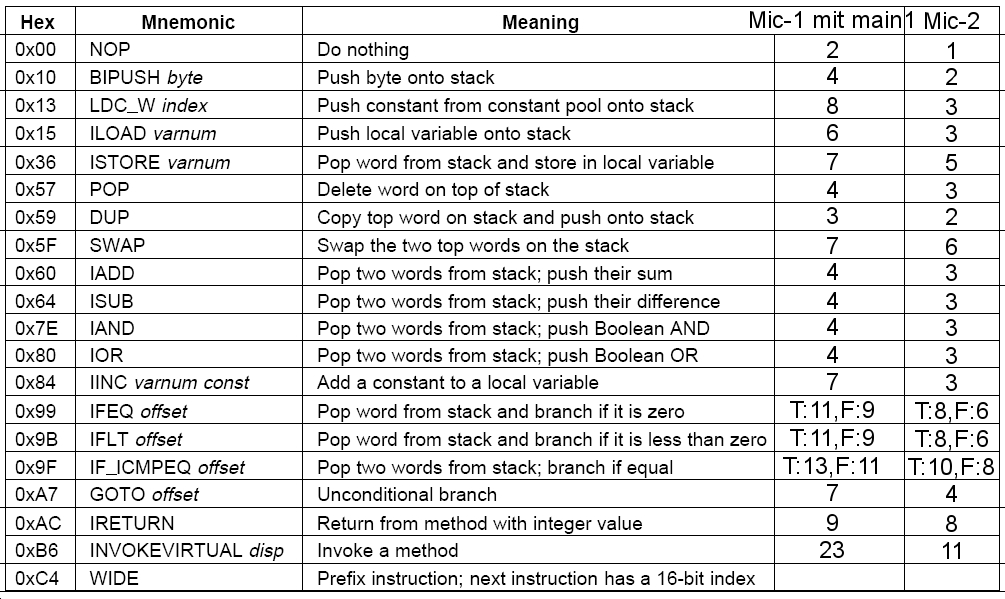
\includegraphics[width=\textwidth]{ALU-Operationen} 

\minisec{Mic-1}
Jede Mikroinstruktion zeigt auf die folgende im Steuerspeicher, am Ende der Instruktion Verweis auf Main1

\minisec{Mic-2}
Einfädeln von Main1 in die Mikroinstruktionen, vollständiger A-Bus, Instruction Fetch Unit (Hochzählen von PC)\\
Prefetch: Puffern des Instruktionsstromes in Schieberegister: \\
Endlicher Automat (Mindestgröße= Wortgröße + längste Instruktion/Operand -1) z.B. bei IJVM 4+2-1 = 5 

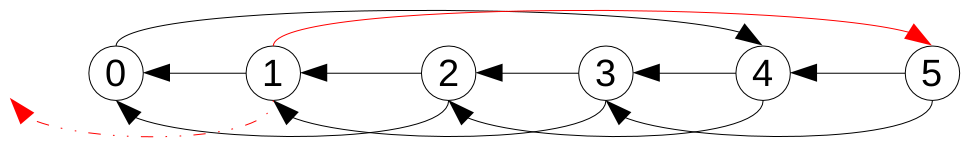
\includegraphics[width=\textwidth]{IFU}

\minisec{Mic-3}
3-stufige Pipeline: Lesen, ALU, Schreiben (RAW-Abhängigkeiten der Mikroinstruktionen beachten) \\ \\
